\documentclass{article}

% Packages for formatting
\usepackage[margin=1in]{geometry}
\usepackage{fancyhdr}
\usepackage{enumerate}
\usepackage{graphicx}
\usepackage{kotex}
\usepackage{amsmath}
\usepackage{amsthm}
\usepackage{algorithm2e,setspace}
\usepackage{algpseudocode}
\usepackage{xcolor}
\usepackage{amssymb}

% Fonts
\usepackage[T1]{fontenc}
\usepackage[utf8]{inputenc}
\usepackage{newpxtext,newpxmath}
\usepackage{sectsty}

% Define colors
\definecolor{blue1}{HTML}{0077c2}
\definecolor{blue2}{HTML}{00a5e6}
\definecolor{blue3}{HTML}{b3e0ff}
\definecolor{blue4}{HTML}{00293c}
\definecolor{blue5}{HTML}{e6f7ff}

\definecolor{thmcolor}{RGB}{231, 76, 60}
\definecolor{defcolor}{RGB}{52, 152, 219}
\definecolor{lemcolor}{RGB}{155, 89, 182}
\definecolor{corcolor}{RGB}{46, 204, 113}
\definecolor{procolor}{RGB}{241, 196, 15}

\usepackage{color,soul}
\usepackage{soul}
\newcommand{\mathcolorbox}[2]{\colorbox{#1}{$\displaystyle #2$}}
\usepackage{cancel}
\newcommand\crossout[3][black]{\renewcommand\CancelColor{\color{#1}}\cancelto{#2}{#3}}
\newcommand\ncrossout[2][black]{\renewcommand\CancelColor{\color{#1}}\cancel{#2}}

\usepackage{hyperref}
\usepackage{booktabs}

% Chapter formatting
\definecolor{titleblue}{RGB}{0,53,128}
\usepackage{titlesec}
\titleformat{\section}
{\normalfont\sffamily\Large\bfseries\color{titleblue!100!gray}}{\thesection}{1em}{}
\titleformat{\subsection}
{\normalfont\sffamily\large\bfseries\color{titleblue!50!gray}}{\thesubsection}{1em}{}

%Tcolorbox
\usepackage[most]{tcolorbox}

%Tikzpicture
\usepackage{pgfplots}
\usepgfplotslibrary{polar}
%\pgfplotsset{compat=1.17}
\usepackage{tikz-cd}
\usetikzlibrary{positioning}
\usetikzlibrary{angles, quotes}

% Header and footer formatting
\pagestyle{fancy}
\fancyhead{}
\fancyhf{}
\rhead{Student ID: 20192250\quad Name: 지용현}%\rule{3cm}{0.4pt}}
\lhead{\textcolor{blue2}{\textbf{CA\hspace{4pt} 2023-spring-Final}}}
% Define footer
\newcommand{\footer}[1]{
	\begin{flushright}
		\vspace{2em}
		
\includegraphics[width=2cm]{school_logo.jpg} \\
		\vspace{1em}
		\textcolor{blue2}{\small\textbf{#1}}
	\end{flushright}
}
%\rfoot{\large Department of Information Security, Cryptogrphy and Mathematics, Kookmin Uni.
\includegraphics[height=1.5cm]{school_logo.jpg}}
\fancyfoot{}
\fancyfoot[C]{-\thepage-}

\newcommand{\ie}{\textnormal{i.e.}}
\newcommand{\rsa}{\mathsf{RSA}}
\newcommand{\rsacrt}{\mathsf{RSA}\textendash\mathsf{CRT}}
\newcommand{\inv}[1]{#1^{-1}}

\usepackage{amsthm}
\newtheorem{axiom}{Axiom}[section]
\newtheorem{theorem}{Theorem}
\newtheorem*{theorem*}{Theorem}
\newtheorem{proposition}[theorem]{Proposition}
\newtheorem{corollary}{Corollary}[theorem]
\newtheorem*{corollary*}{Corollary}
\newtheorem{lemma}[theorem]{Lemma}
\newtheorem*{lemma*}{Lemma}

\theoremstyle{definition}
\newtheorem{definition}{Definition}
\newtheorem*{definition*}{Definition}
\newtheorem{remark}{Remark}
\newtheorem{exercise}{Exercise}[section]

%New Command
\newcommand{\set}[1]{\left\{#1\right\}}
\newcommand{\N}{\mathbb{N}}
\newcommand{\Z}{\mathbb{Z}}
\newcommand{\Q}{\mathbb{Q}}
\newcommand{\R}{\mathbb{R}}
\newcommand{\C}{\mathbb{C}}
\newcommand{\F}{\mathbb{F}}
\newcommand{\nbhd}{\mathcal{N}}
\newcommand{\Log}{\operatorname{Log}}
\newcommand{\Arg}{\operatorname{Arg}}
\newcommand{\pv}{\operatorname{P.V.}}

\newcommand{\of}[1]{\left( #1 \right)} 
\newcommand{\abs}[1]{\left\lvert #1 \right\rvert}
\newcommand{\norm}[1]{\left\| #1 \right\|}

\newcommand{\sol}{\textcolor{magenta}{\bf Sol}}
\newcommand{\conjugate}[1]{\overline{#1}}

\newcommand{\res}{\textnormal{res}}

\renewcommand{\Re}{\operatorname{Re}}
\renewcommand{\Im}{\operatorname{Im}}

\begin{document}
	\pagenumbering{arabic}
	\begin{center}
		\huge\textbf{Complex Analysis - Final}\\
		\vspace{0.5em}
	\end{center}
	
	\begin{enumerate}[\bf 1.]
		\item Find the keyword most closely related to the following sentences:
		\begin{enumerate}
			\item If the complex function $f(z)$ is differentiable in an open set containing a region enclosed by the curve $C$, then $\int_{C}f(z)dz=0$.\[
			\boxed{\text{Cauchy-Goursat Theorem}}
			\]
			\item If the complex function $f(z)$ is differentiable in the region $\abs{z} > 1$, it can be expressed as a power series.\[
			\boxed{\text{Laurent Series}}
			\]
			\item Each point on the complex plane corresponds one-to-one with a point on a sphere, excluding the north pole.\[
			\boxed{\text{Riemann Sphere}}
			\]
			\item All solutions to $2z^5 - 6z^2 + z + 1 = 0$ exist within the region $\abs{z} < 2$.\[
			\boxed{\text{Rouch\'{e}'s Theorem}}
			\]
			\item If the function $f(z)$, which is differentiable on the entire complex plane, satisfies $\abs{f(z)}\leq 1$, then $f(z)$ is a constant function. \[
			\boxed{\text{Liouville's Theorem}}
			\]
			\item If the complex function $f(z)$ is differentiable in an open set containing a region enclosed by the curve $C$, the value of the function inside the curve is determined by the value of the function on the curve. \[
			\boxed{\text{Cauchy Integral Formula}}
			\]
			\item For a harmonic function $h(x, y)$ defined on an open set including the unit circle $U$ and its interior, the value of the function inside the unit circle is determined by the value of the function on the unit circle. \[
			\boxed{\text{Poisson Integral Formula}}
			\]
			\item A continuous function $f(z)$ defined on an open region $D$ is differentiable if it satisfies the condition that $\int_{C}f(z)dz=0$ for all closed curves $C$ in the region $D$. \[
			\boxed{\text{Morera's Theorem}}
			\]
			\item There exists a differentiable complex function that maps a simply connected domain (not the entire complex plane) one-to-one to the interior of the unit circle. \[
			\boxed{\text{Riemann Mapping Theorem}}
			\]
			\item For all polynomials $P(z)$ with complex coefficients, the equation $P(z) = 0$ has a complex solution. \[
			\boxed{\text{Fundamental Theorem of Algebra}}
			\]
		\end{enumerate}
		\newpage
		\item What is the integral \[
		\int_Cz\ dz
		\] over the line segment $C$ from the origin $z_1 = 0$ to $z_2 = 1 + i$?
		\begin{proof}[\sol]
			Let $z=(1+i)t$ with $t\in[0,1]$. \begin{center}
				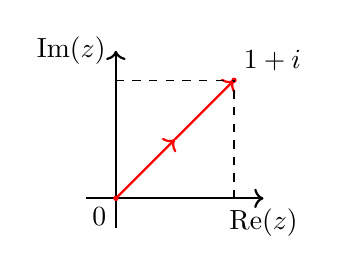
\begin{tikzpicture}[scale=1.5]
				\draw[thick,->] (-.25,0) -- (1.25,0) node[below] {$\Re(z)$};
				\draw[thick,->] (0,-.25) -- (0,1.25) node[left] {$\Im(z)$};
				
				\draw[->, thick, red] (0,0) -- (.5,.5) ;
				\draw[->, thick, red] (.5,.5) -- (1,1) ;
				\filldraw[red] (1,1) circle (.5pt) node[above right, black] {$1+i$};
				\filldraw[red] (0,0) circle (.5pt) node[below left, black] {$0$};
				
				\draw[dashed] (0,1) -- (1,1);
				\draw[dashed] (1,0) -- (1,1);
				\end{tikzpicture}
			\end{center} Since $z=(1+i)t\Rightarrow dz=(1+i)dt$, we have \[
			\int_C z\ dz=\int_0^1(1+i)t\ (1+i)dt=(1+i)^2\int_0^1t\ dt=2i\cdot\frac{1}{2}=i.
			\]
		\end{proof}
		\vspace{8pt}
		\item What is the integral \[
		\int_C \frac{1}{(z-1)^2}\ dz
		\] over the curve $C$ which traverses the circle $\abs{z} = 2$ in a counterclockwise direction?
		\begin{proof}[\sol]
			Let $f(z)=(z-1)^{-2}$. \begin{center}
				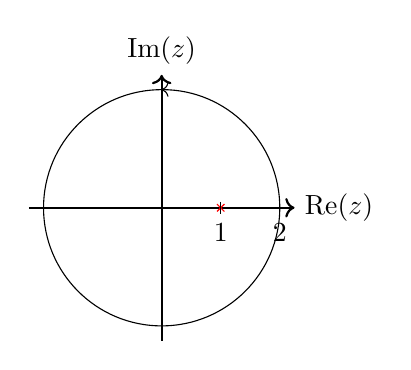
\begin{tikzpicture}[scale=.75]
				\draw[thick,->] (-2.25,0) -- (2.25,0) node[right] {$\Re(z)$};
				\draw[thick,->] (0,-2.25) -- (0,2.25) node[above] {$\Im(z)$};
				
				\draw[->] (2,0) arc (0:90:2);
				\draw[-] (0,2) arc (90:360:2);
				\draw[red, mark size=2.5pt] plot[mark=x] coordinates{(1,0)};
				\draw[] (1,.1) -- (1,-.1) node[below] {$1$};
				\draw[] (2,.1) -- (2,-.1) node[below] {$2$};
				\end{tikzpicture}
			\end{center} By residue theorem, we have\[
			\oint_C\frac{1}{(z-1)^2}\ dz=2\pi i\cdot\res(f,1)=0.
			\]
		\end{proof}
		\vspace{8pt}
		\item What are the partial derivatives of the complex function \[
		f(x,y)=u(x,y)+iv(x,y)=\begin{cases}
		\frac{\of{\conjugate{z}}^2}{z} &:z\neq0,\\
		0 &:z=0.
		\end{cases}
		\] at the origin?
		\begin{proof}[\sol]
			Let $z=x+iy$ then \begin{align*}
			\frac{\of{\conjugate{z}}^2}{z}=\frac{(x-iy)^2}{x+iy}&=\frac{(x-iy)^3}{x^2+y^2}\\
			&=\frac{x^3+3x^2(-iy)+3x(-iy)^2+(-iy)^3}{x^2+y^2}\\
			&=\frac{x^3-3x^2yi-3xy^2+iy^3}{x^2+y^2}\\
			&=\frac{x^3-3xy^2}{x^2+y^2}+i\frac{y^3-3x^2y}{x^2+y^2}.
			\end{align*} Here, let \[
			u(x,y)=\frac{x^3-3xy^2}{x^2+y^2}\quad\text{and}\quad v(x,y)=\frac{y^3-3x^2y}{x^2+y^2}.
			\] Then \begin{align*}
			u_x(0,0)&=\lim\limits_{h\to 0}\frac{u(h,0)-u(0,0)}{h}=\lim\limits_{h\to 0}\frac{\frac{h^3-0}{h^2+0}}{h}=1,\\
			v_x(0,0)&=\lim\limits_{h\to 0}\frac{v(h,0)-v(0,0)}{h}=\lim\limits_{h\to 0}\frac{\frac{0}{h^2}}{h}=0.
			\end{align*}
		\end{proof}
		\vspace{8pt}
		\item What is the result of the integral \[
		\int_C \frac{1}{z(z-2)^4}\ dz
		\] over the curve $C$ which traverses the circle $\abs{z-2} = 1$ in a counterclockwise direction?
		\begin{proof}[\sol]
			Let $f(z)=\frac{1}{z}$. Note that \[
			f^{(1)}(z)=-1z^{-2},\quad f^{(2)}(z)=2z^{-3},\quad f^{(3)}(z)=-6z^{-4}.
			\] \begin{center}
				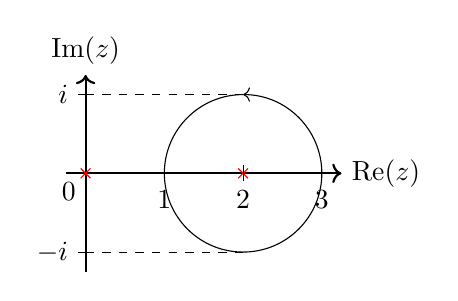
\begin{tikzpicture}[scale=1]
				\draw[thick,->] (-.25,0) -- (3.25,0) node[right] {$\Re(z)$};
				\draw[thick,->] (0,-1.25) -- (0,1.25) node[above] {$\Im(z)$};
				
				\draw[->] (3,0) arc (0:90:1);
				\draw[-] (2,1) arc (90:360:1);
				\draw[red, mark size=2.5pt] plot[mark=x] coordinates{(2,0)};
				\draw[red, mark size=2.5pt] plot[mark=x] coordinates{(0,0)};
				\node[below left] {$0$};
				\draw[] (1,.1) -- (1,-.1) node[below] {$1$};
				\draw[] (2,.1) -- (2,-.1) node[below] {$2$};
				\draw[] (3,.1) -- (3,-.1) node[below] {$3$};
				
				\draw[] (.1,1) -- (-.1,1) node[left] {$i$};
				\draw[] (.1,-1) -- (-.1,-1) node[left] {$-i$};
				
				\draw[dashed] (0,1) -- (2,1);
				\draw[dashed] (0,-1) -- (2,-1);
				\end{tikzpicture}
			\end{center} Recall that the Cauchy Integral Formula: \[
			f^{(n)}(z_0)=\frac{n!}{2\pi i}\oint_C\frac{f(z)}{(z-z_0)^{n+1}}\ dz.
			\] Thus, \[
			f^{(3)}(2)=\frac{3!}{2\pi i}\oint_C\frac{1/z}{(z-2)^4}\ dz=-6\cdot2^{-4}\implies\oint_C\frac{1/z}{(z-2)^4}\ dz=\frac{2\pi i}{6}\cdot\of{-\frac{6}{16}}=-\frac{\pi i}{8}.
			\]
		\end{proof}
		\item What is the value of the integral \[
		\int_C z^2\exp\of{\frac{1}{z}}\ dz
		\] over the curve $C$ which traces the circle $\abs{z} = 2$ in a counterclockwise direction?
		\begin{proof}[\sol]
			Let $f(z)=z^2\exp(1/z)$ then \begin{align*}
			f(z)=z^2\exp\of{\frac{1}{z}}&=z^2\of{1+\of{\frac{1}{z}}+\frac{1}{2!}\of{\frac{1}{z}}^2+\frac{1}{3!}\of{\frac{1}{z}}^3+\cdots}\\
			&=z^2+z+\frac{1}{2!}+\frac{1}{3!}\frac{1}{z}+\cdots.
			\end{align*}\begin{center}
				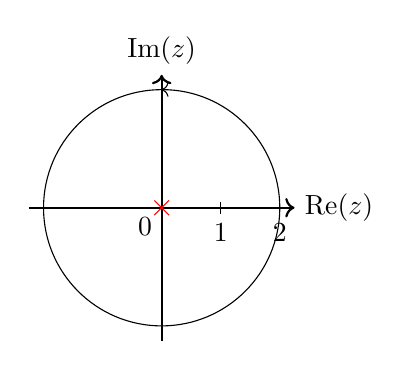
\begin{tikzpicture}[scale=.75]
				\draw[thick,->] (-2.25,0) -- (2.25,0) node[right] {$\Re(z)$};
				\draw[thick,->] (0,-2.25) -- (0,2.25) node[above] {$\Im(z)$};
				
				\draw[->] (2,0) arc (0:90:2);
				\draw[-] (0,2) arc (90:360:2);
				\draw[red, mark size=5pt] plot[mark=x] coordinates{(0,0)};
				\node[below left] {$0$};
				\draw[] (1,.1) -- (1,-.1) node[below] {$1$};
				\draw[] (2,.1) -- (2,-.1) node[below] {$2$};
			\end{tikzpicture}
			\end{center} \[
			\oint_C\ z^2\exp\of{\frac{1}{z}}\ dz=2\pi i\cdot\res(f,0)=2\pi i\cdot\frac{1}{3!}=\frac{\pi i}{6}.
			\]
		\end{proof}
		\vspace{8pt}
		\item What is the value of the integral \[
		\int_C\frac{e^z}{z-1}\ dz
		\] over the curve $C$ which traces the circle $\abs{z} = 1/2$ in a counterclockwise direction?
		\begin{proof}[\sol]
			\ \begin{center}
				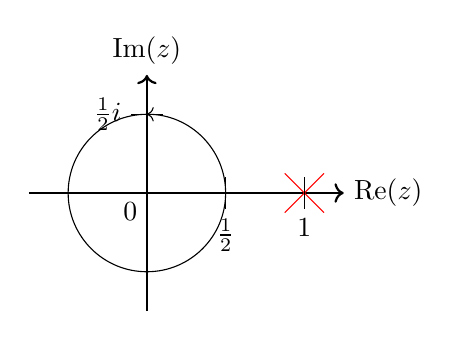
\begin{tikzpicture}[scale=2]
				\draw[thick,->] (-.75,0) -- (1.25,0) node[right] {$\Re(z)$};
				\draw[thick,->] (0,-.75) -- (0,.75) node[above] {$\Im(z)$};
				
				\draw[->] (.5,0) arc (0:90:.5);
				\draw[-] (0,.5) arc (90:360:.5);
				\draw[red, mark size=5pt] plot[mark=x] coordinates{(1,0)};
				\node[below left] {$0$};
				\draw[] (.5,.1) -- (.5,-.1) node[below] {$\frac{1}{2}$};
				\draw[] (1,.1) -- (1,-.1) node[below] {$1$};
				
				\draw[] (.1,.5) -- (-.1,.5) node[left] {$\frac{1}{2}i$};
				\end{tikzpicture}
			\end{center} By the Cauchy-Goursat Theorem, $$\oint_C\frac{e^z}{z-1}\ dz=0$$.
		\end{proof}
		\item What is the value of the following integral \[
		\frac{1}{2\pi i}\int_C\frac{z^{2021}}{z^{2022}+1}\ dz
		\] over the curve $C$ which traces the circle $\abs{z} = 2$ in a counterclockwise direction?
		\begin{proof}[\sol]
			\ \begin{tcolorbox}[colback=white,colframe=thmcolor,arc=5pt,title={\color{white}\bf Argument Principle}]
				Let $f$ is holomorphic in a simple closed curve $C$. Then \[
				\frac{1}{2\pi i}\oint_C\frac{f'(z)}{f(z)}\ dz=Z-P,
				\] where $Z$ denote the number of zeroes of $f$ in $C$ and $P$ denote the number of poles of $f$ in $C$.
			\end{tcolorbox}
			Let $f(z):z^{2022}+1$ then $f'(z)=2022\cdot z^{2021}$. Thus \[
			\frac{1}{2\pi i}\oint_C\frac{2022 z^{2021}}{z^{2022}+1}\ dz = Z-P=2022-0=2022.
			\] Thus $\displaystyle=\frac{1}{2\pi i}\oint_C\frac{z^{2021}}{z^{2022}+1}\ dz =1$.
		\end{proof}
		\item How many roots does the equation $z^7 - 5z^3 + 12 = 0$ have inside the circle $\abs{z} = 1$?
		\begin{proof}[\sol]
			
		\end{proof}
		\newpage
		\item For the complex function $f(z)=\displaystyle\frac{3}{2+z-z^2}$,
		\begin{enumerate}
			\item When the Laurent series of $f$ is written as \[
			f(z)=\sum_{n=0}^{\infty}a_nz^n+\sum_{n=1}^\infty\frac{b_n}{z^n}
			\] in the region $1<\abs{z}<2$, what is the value of $a_0+a_1+b_1$?
			\vspace{4pt}
			\item What is the value of the residue $\res(f,2)$ of $f(z)$ at $z=2$?
		\end{enumerate}
		\begin{proof}[\sol]
			\begin{enumerate}[(a)]
				\item Note that \[
				f(z)=\frac{3}{2+z-z^2}=\frac{-3}{z^2-z-2}=\frac{-3}{(z-2)(z+1)}=\frac{-1}{z-2}+\frac{1}{z+1}.
				\] Then \[
				\begin{cases}
				\displaystyle\frac{-1}{z-2}=\frac{1/2}{1-z/2}=\frac{1}{2}\of{1+\of{\frac{z}{2}}+\of{\frac{z}{2}}^2+\cdots} &\because\abs{z}<2,\\
				\\
				\displaystyle\frac{1}{z+1}=\frac{1/z}{1-(-1/z)}=\frac{1}{z}\of{1+\of{-\frac{1}{z}}+\of{-\frac{1}{z}}^2+\cdots} &\because\abs{z}>1.\\
				\end{cases}
				\] Thus \begin{align*}
				f(z)&=\of{\frac{1}{2}+\frac{1}{2^2}z+\frac{1}{2^3}z^2+\cdots}+\of{\frac{1}{z}-\frac{1}{z^2}+\frac{1}{z^3}-\cdots}\\
				&=\sum_{n=0}^\infty\frac{1}{2^{n+1}}z^n+\sum_{n=1}^\infty(-1)^{n+1}z^{-n}.
				\end{align*} Hence $a_0+a_1+b_1=1/2+1/4+1=7/4$.
				\vspace{4pt}
				\item Note that \begin{align*}
				f(z)=\frac{-1}{z-2}+\frac{1}{z+1}&=\frac{-1}{z-2}+\sum_{n=0}^{\infty}c_n(z-2)^n,
				\end{align*} since $1/(z+1)$ is holomorphic in $\abs{z-2}<\varepsilon$ for all $\varepsilon>0$. Thus $\res(f,2)=-1$.
			\end{enumerate}
		\end{proof}
		\newpage
		\item Find the following improper integral: \[
		\int_0^{\infty}\frac{1+x^2}{1+x^4}\ dx.
		\]
		\begin{proof}[\sol]
			Let $f(z)=\displaystyle\frac{1+z^2}{1+z^4}$. Let $C=C_R+I_R$ as follows:
			\begin{center}
				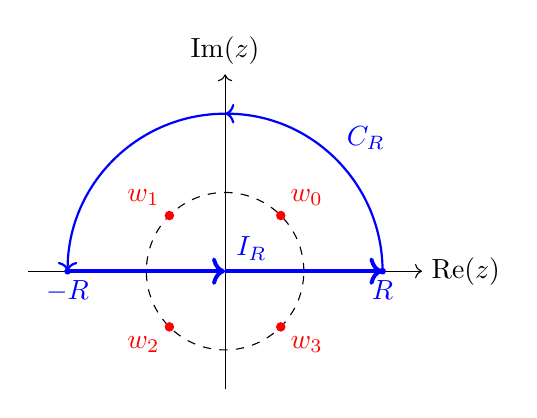
\begin{tikzpicture}[scale=1]
				%\draw[white, pattern={Lines[angle=45,distance={12pt/sqrt(3)}]}, pattern color=blue] (2,0) arc (0:180:2) node[midway, above right] {};
				% draw axes
				\draw[->] (-2.5,0) -- (2.5,0) node[right] {$\Re(z)$};
				\draw[->] (0,-1.5) -- (0,2.5) node[above] {$\Im(z)$};
				% add arrow
				%\draw[->] (0,0) -- (1,1) node[midway, above left] {};
				\draw[dashed] (1,0) arc (0:360:1);
				% draw point
				\filldraw[red] ({1/sqrt(2)},{1/sqrt(2)}) circle (1.5pt) node[anchor=south west] {$w_0$};
				\filldraw[red] (-{1/sqrt(2)},{1/sqrt(2)}) circle (1.5pt) node[anchor=south east] {$w_1$};
				\filldraw[red] (-{1/sqrt(2)},-{1/sqrt(2)}) circle (1.5pt) node[anchor=north east] {$w_2$};
				\filldraw[red] ({1/sqrt(2)},-{1/sqrt(2)}) circle (1.5pt) node[anchor=north west] {$w_3$};
				\filldraw[blue] (2,0) circle (1pt) node[anchor=north] {$R$};
				\filldraw[blue] (-2,0) circle (1pt) node[anchor=north] {$-R$};
				
				\draw[line width=0.5mm, ->, thick, blue] (2,0) arc (0:90:2) node[midway, above right] {$C_R$};
				\draw[line width=0.5mm, ->, thick, blue] (0,2) arc (90:180:2) node[midway, left] {};
				\draw[line width=0.5mm, blue, ->] (-2,0) -- (0,0) node[above right] {$I_R$};
				\draw[line width=0.5mm, blue, ->] (0,0) -- (2,0) node[above right] {};
				\end{tikzpicture}
			\end{center} then \begin{align*}
			\res(f,w_0)=\lim\limits_{z\to w_0}(z-w_0)f(z)=\lim\limits_{z\to w_0}\frac{z-w_0+z^3-w_0z^2}{1+z^4}=\lim\limits_{z\to w_0}\frac{3z^2-2zw_0+1}{4z^3}=\frac{1}{4}\of{w_0^{-1}+w_0^{-3}},
		\end{align*} that is, \begin{align*}
		\res(f,e^{\frac{\pi}{4}i})&=\frac{1}{4}\of{e^{-\frac{\pi}{4}i}+e^{-\frac{3\pi}{4}i}}=\frac{1}{4}\of{\frac{1}{\sqrt{2}}-\frac{i}{\sqrt{2}}-\frac{1}{\sqrt{2}}-\frac{i}{\sqrt{2}}}=-\frac{i}{2\sqrt{2}}\\
		\res(f,e^{\frac{3\pi}{4}i})&=\frac{1}{4}\of{e^{-\frac{3\pi}{4}i}+e^{-\frac{9\pi}{4}i}}=-\frac{i}{2\sqrt{2}}.
		\end{align*} And so \[
		\oint_Cf(z)\ dz=2\pi i\of{\res(f,w_0)+\res(f,w_1)}=2\pi i\cdot 2\cdot\frac{-i}{2\sqrt{2}}=\sqrt{2}\pi.
		\] Consider \[
		\oint_C f(z)\ dz=\underbrace{\int_{C_R}f(z)\ dz}_{=\text{(1)}}+\underbrace{\int_{I_R}f(z)\ dz}_{=\text{(2)}}.
		\] \begin{enumerate}[(1)]
			\item Since $\abs{f(z)}=\abs{\frac{1+z^2}{1+z^4}}\leq\frac{\abs{z}^2-1}{\abs{z}^4-1}=\frac{R^2-1}{R^4-1}$, \[
			\abs{\int_{C_R}f(z)\ dz}\leq\frac{R^2-1}{R^4-1}\cdot\pi R\to 0\quad\text{as}\quad R\to 0.
			\]
			\item $\displaystyle\int_{I_R}f(z)\ dz=\int_{-R}^{R}\frac{1+x^2}{1+x^4}\ dx\to\int_{-\infty}^{\infty}\frac{1+x^2}{1+x^4}\ dx$\quad as\quad $R\to\infty$.
		\end{enumerate}
		By (1) and (2), \begin{align*}
		\lim\limits_{R\to\infty}\oint_C f(z)\ dz=\int_{-\infty}^{\infty}\frac{1+x^2}{1+x^4}\ dx&=2\int_{0}^{\infty}\frac{1+x^2}{1+x^4}\ dx\quad\text{$\because$ $f$ is even}\\
		&=\sqrt{2}\pi.
		\end{align*} Hence $\displaystyle\int_{0}^{\infty}\frac{1+x^2}{1+x^4}\ dx=\frac{\sqrt{2}}{2}\pi$.
		\end{proof}
		\item Find the following improper integral: \[
		\int_{-\infty}^{\infty}\frac{x\sin x}{x^2+1}\ dx.
		\]
		\begin{proof}[\sol]
			Let $\displaystyle f(z):=\frac{z}{z^2+1}=\frac{z}{(z-i)(z+i)}$, and let $
			\displaystyle f(z)e^{iz}=\frac{\phi(z)}{z-i}$ with $\displaystyle\phi(z)=\frac{ze^{iz}}{z+i}$. Here $\phi$ is analytic at $z=i$. Let $C:=C_R+I_R$: \begin{center}
				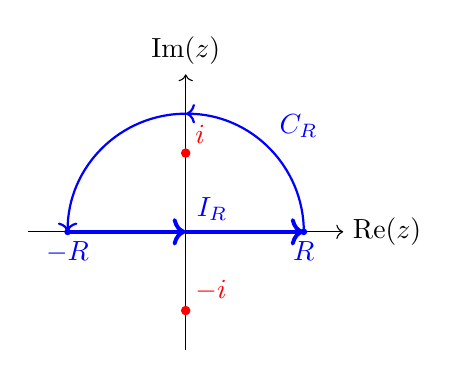
\begin{tikzpicture}[scale=1]
				% draw axes
				\draw[->] (-2,0) -- (2,0) node[right] {$\Re(z)$};
				\draw[->] (0,-1.5) -- (0,2) node[above] {$\Im(z)$};
				% add arrow
				%\draw[->] (0,0) -- (1,1) node[midway, above left] {};
				% draw point
				\filldraw[red] (0,1) circle (1.5pt) node[anchor=south west] {$i$};
				\filldraw[red] (0,-1) circle (1.5pt) node[anchor=south west] {$-i$};
				\filldraw[blue] (1.5,0) circle (1pt) node[anchor=north] {$R$};
				\filldraw[blue] (-1.5,0) circle (1pt) node[anchor=north] {$-R$};
				
				\draw[line width=0.5mm, ->, thick, blue] (1.5,0) arc (0:90:1.5) node[midway, above right] {$C_R$};
				\draw[line width=0.5mm, ->, thick, blue] (0,1.5) arc (90:180:1.5) node[midway, left] {};
				\draw[line width=0.5mm, blue, ->] (-1.5,0) -- (0,0) node[above right] {$I_R$};
				\draw[line width=0.5mm, blue, ->] (0,0) -- (1.5,0) node[above right] {};
				\end{tikzpicture}
			\end{center} then \[
			\res\of{f(z)e^{iz},i}=\res\of{\frac{\phi(z)}{z-i},i}=\phi(i)=\frac{ie^{-1}}{2i}=\frac{1}{2e}.
			\] Consider $$
			\displaystyle\oint_C f(z)e^{iz}\ dz=\underbrace{\int_{C_R}f(z)e^{iz}\ dz}_{=(1)}+\underbrace{\int_{I_R}f(z)e^{iz}\ dz}_{=(2)}.
			$$ \begin{enumerate}[(1)]
				\item Since $\displaystyle \abs{f(z)}=\abs{\frac{z}{z^2+1}}\leq\frac{\abs{z}}{\abs{z}^2-1}=\frac{R}{R^2-1}=:M_R$, $$\lim\limits_{R\to\infty}\int_{C_R}f(z)e^{iz}\ dz=0$$ by Jordan's Lemma.
				\item \[
				\int_{I_R}f(z)e^{iz}\ dz=\int_{-R}^R\frac{x}{x^2+1}\cos x\ dx+i\int_{-R}^R\frac{x}{x^2+1}\sin x\ dx.
				\]
			\end{enumerate}
			By (1) and (2) \begin{align*}
			\lim\limits_{R\to\infty}\oint_C f(z)e^{iz}\ dz&=\int_{-\infty}^{\infty}\frac{x}{x^2+1}\cos x\ dx+i\int_{-\infty}^{\infty}\frac{x}{x^2+1}\sin x\ dx\\
			&=2\pi i\cdot\res\of{f(z)e^{iz}, i}\\
			&=\frac{\pi}{e}i.
			\end{align*} Hence \[
			\int_{-\infty}^{\infty}\frac{x}{x^2+1}\sin x\ dx=\frac{\pi}{e}.
			\]
		\end{proof}
		\newpage
		\item 
		Define the regions $D_1$ and $D_2$ on the complex plane as follows:\[
		D_1:=\set{z\in\C:\abs{z-2}<2},\quad D_2:=\set{z\in\C:\abs{z-1}>1}.
		\]
		\begin{enumerate}[(a)]
			\item Find the linear fractional function $f(z)=\displaystyle\frac{az+b}{cz+d}$ that maps $z_1$, $z_2$, $z_3$ to $w_1$, $w_2$, $w_3$ respectively as follows: \[
			\begin{cases}
			z_1=0\mapsto w_1=\infty,\\
			z_2=2\mapsto w_2=i,\\
			z_3=4\mapsto w_3=0.
			\end{cases}
			\]
			\item Represent on the complex plane the region to which $f(z)$ maps the region $D_1\cap D_2$.
		\end{enumerate}
		\begin{proof}[\sol]
			\ \begin{center}
				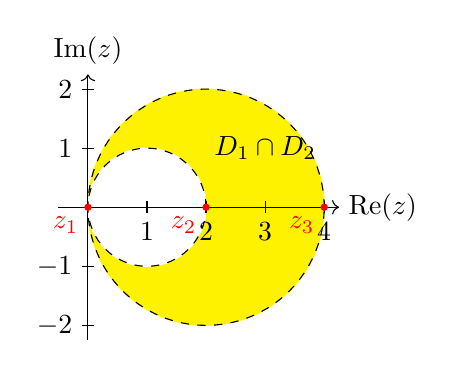
\begin{tikzpicture}[scale=.75]
				% D_1 and D_2
				\filldraw[yellow] (4,0) arc (0:360:2) node[above right, black] {};
				\filldraw[white] (2,0) arc (0:360:1) node[above, black] {};
				\draw[dashed] (4,0) arc (0:360:2) node[right, black] {};
				\draw[dashed] (2,0) arc (0:360:1) node[left, black] {};
				\node[] at (3,1) {$D_1\cap D_2$};
				
				% draw axes
				\draw[->] (-.5,0) -- (4.25,0) node[right] {$\Re(z)$};
				\draw[->] (0,-2.25) -- (0,2.25) node[above] {$\Im(z)$};
				
				% Take Coordinates
				\foreach \i in {1,2,...,4}
				\draw[] (\i,.1)--(\i,-.1) node[below] {$\i$};%x-axis
				\foreach \i in {-2,-1,1,2}
				\draw[] (.1,\i)--(-.1,\i) node[left] {$\i$};%y-axis
				
				\filldraw[red] (0,0) circle (1.5pt) node[below left] {$z_1$};
				\filldraw[red] (2,0) circle (1.5pt) node[below left] {$z_2$};
				\filldraw[red] (4,0) circle (1.5pt) node[below left] {$z_3$};
				\end{tikzpicture}
			\end{center}
			\begin{enumerate}[(a)]
				\item Let \[
				f(z):=\frac{z-z_3}{z-z_1}\cdot\alpha=\frac{z-4}{z}\cdot\alpha.
				\] Since $i=w_2=f(z_2)=f(2)$, \[
				f(2)=-\alpha=i\implies\alpha=-i.
				\] Thus \[
				f(z)=-i\cdot\frac{z-4}{z}=\frac{4i-iz}{z}.
				\]
				\item \ \begin{figure}[h!]
					\centering
					\begin{minipage}{.4\textwidth}
						\centering
						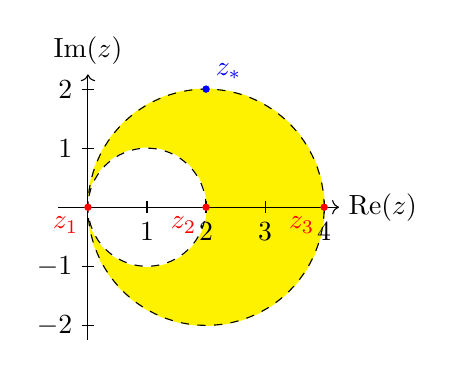
\begin{tikzpicture}[scale=.75]
						% D_1 and D_2
						\filldraw[yellow] (4,0) arc (0:360:2) node[above right, black] {};
						\filldraw[white] (2,0) arc (0:360:1) node[above, black] {};
						\draw[dashed] (4,0) arc (0:360:2) node[right, black] {};
						\draw[dashed] (2,0) arc (0:360:1) node[left, black] {};
						
						% draw axes
						\draw[->] (-.5,0) -- (4.25,0) node[right] {$\Re(z)$};
						\draw[->] (0,-2.25) -- (0,2.25) node[above] {$\Im(z)$};
						
						% Take Coordinates
						\foreach \i in {1,2,...,4}
						\draw[] (\i,.1)--(\i,-.1) node[below] {$\i$};%x-axis
						\foreach \i in {-2,-1,1,2}
						\draw[] (.1,\i)--(-.1,\i) node[left] {$\i$};%y-axis
						
						\filldraw[red] (0,0) circle (1.5pt) node[below left] {$z_1$};
						\filldraw[red] (2,0) circle (1.5pt) node[below left] {$z_2$};
						\filldraw[red] (4,0) circle (1.5pt) node[below left] {$z_3$};
						\filldraw[blue] (2,2) circle (1.5pt) node[above right] {$z_*$};
						\end{tikzpicture}
					\end{minipage}\quad
					$\xrightarrow{f}$\quad
					\begin{minipage}{.4\textwidth}
						\centering
						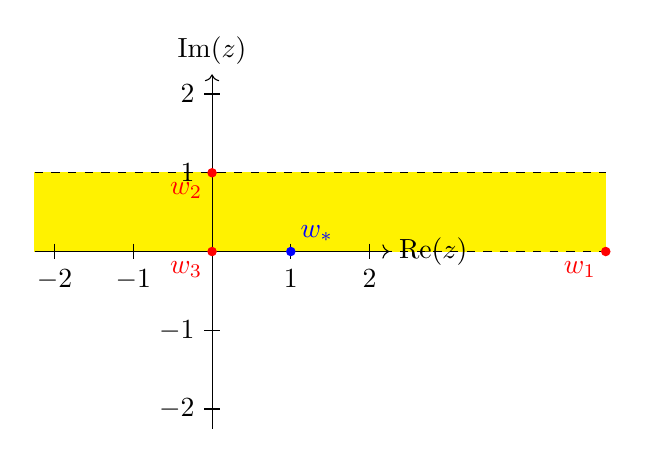
\begin{tikzpicture}[scale=1]
						\filldraw[yellow] (-2.25,0) rectangle (5,1) node[above right, black] {};
						\draw[dashed] (-2.25,1) -- (5,1) node[right, black] {};
						\draw[dashed] (-2.25,0) -- (5,0) node[left, black] {};
						
						% draw axes
						\draw[->] (-2.25,0) -- (2.25,0) node[right] {$\Re(z)$};
						\draw[->] (0,-2.25) -- (0,2.25) node[above] {$\Im(z)$};
						
						% Take Coordinates
						\foreach \i in {-2,-1,1,2}
						\draw[] (\i,.1)--(\i,-.1) node[below] {$\i$};%x-axis
						\foreach \i in {-2,-1,1,2}
						\draw[] (.1,\i)--(-.1,\i) node[left] {$\i$};%y-axis
						
						\filldraw[red] (5,0) circle (1.5pt) node[below left] {$w_1$};
						\filldraw[red] (0,1) circle (1.5pt) node[below left] {$w_2$};
						\filldraw[red] (0,0) circle (1.5pt) node[below left] {$w_3$};
						\filldraw[blue] (1,0) circle (1.5pt) node[above right] {$w_*$};
						\end{tikzpicture}
					\end{minipage}
				\end{figure}
			\end{enumerate}
		\end{proof}
	\end{enumerate}
	
	
	\footer{Department of Information Security, Cryptography and Mathematics\\
		College of Science and Technology\\
		Kookmin University}
\end{document}